% !TEX root = Hogwarts_1347.tex

\chapter{The Irish Sea}

The morning arrived without drama. Thomas became aware of it gradually --- the quality of the light through the gap above the curtain, warmer and more direct than the grey seep of the previous days, and then the sound of boots on the deck above, purposeful and unhurried, the ordinary noise of a crew that wasn't managing a crisis.

He lay still for a moment, listening for the ship's motion. The long, rolling swell was still there, but it was gentle now, almost courteous, the Siren moving through the water as though she belonged there.

Pippin made a small, contented sound on his hook.

Thomas got up.

\section*{A Roof Tile for Breakfast}

By the time he reached the main deck, the crew had already been at work for some time. Two long tables had been mounted on the open deck amidships, sturdy and well-secured to cleats bolted into the planking, and benches fixed alongside them. The sky above was a clean, pale blue, the kind that suggests it has been that way for some time and intends to continue. The sun was still low but already warm on the face when you turned toward it. The sea around them was dark and calm, running in slow, easy swells that caught the light along their crests.

Baldwin appeared at his shoulder, blinking behind his spectacles.

\enquote{Oh,} Baldwin said, looking at the sky with the expression of someone revising their expectations upward.

\enquote{Yes,} Thomas agreed.

They found places at the nearer table. Others arrived in ones and twos --- Philippa, who looked at the weather with satisfaction, as though it had made a sensible decision; Celine, who tilted her face toward the sun immediately and closed her eyes for a moment before sitting down; Cecile, who assessed the tables, the benches, and the securing arrangements before sitting down, satisfied that they were adequate.

Breakfast came up from the galley in a wooden crate, and the contrast with the previous mornings was immediate and democratically suffered.

The bread was gone. In its place were ship's biscuits\footnote{A flat, hard bread made from flour, water, and sometimes salt, baked multiple times to remove all moisture. Hard, dry breads of this kind have sustained armies and sailors since antiquity — the Roman military carried a similar provision called \textit{bucellatum}. It required soaking in water or broth to be edible.} --- hard, flat, pale rounds that looked considerably more confident than they had any right to be. Thomas picked one up and discovered it had the density and temperament of a roof tile.

\enquote{You have to soak it,} Cecile said, without looking up. She had already placed hers in her cup and was waiting with the patience of someone who had done this before.

A round-faced boy with rosy cheeks, who had arrived at the table looking entirely cheerful for early morning on the open sea, picked up his biscuit and examined it with an expression of polite scepticism. He took a considered bite.

The sound it produced was architectural.

He set it down carefully. \enquote{Right,} he said, with great composure, reaching for his cup.

Celine laughed. Philippa passed him the pot of hot water.

\enquote{Barnabus Finch,} the boy said, by way of introduction, dunking his biscuit with the composure of a boy who had just learned an important lesson about the sea.

The fresh fruit was also gone. The basket in the centre of the table held honeyed fruits instead --- figs and blackberries suspended in thick golden honey, dates soft and dark at the bottom of their jar, and slices of apple preserved in the same amber sweetness. Philippa took the honeyed apple slices from the smaller basket at the table's end and distributed them without comment, the implicit message being that this was what there was now and should be appreciated accordingly.

The biscuits, once sufficiently soaked, were not exactly good. But they were edible, and the butter that came with them --- heavily salted, preserved for the journey --- improved matters considerably.

The morning settled into itself.

\section*{Up to Four to a Board}

Someone produced a Pachisi board before the cups were cleared, and then another appeared, and by mid-morning four games were running simultaneously on the two tables, the boards laid out in the patches of sun between the cups and the honey jars.

The games enforced their own groupings, up to four to a board, and the groupings produced their own small dramas.

Cassian Sterling played with the unhurried goodwill of a boy whose attention was mostly elsewhere. He moved his pieces correctly and without apparent error, but between turns his gaze drifted upward --- to the rigging, to the horizon, and most frequently to the sky itself, which offered nothing of particular astronomical interest at this hour but seemed to content him anyway. He won the first game by a margin that surprised everyone, including apparently himself, having spent most of it studying a formation of clouds to the northwest.

\enquote{You weren't even watching the board,} Aiko said.

\enquote{I was watching it,} Cassian said, still looking at the clouds.

Aiko Sanada played the way she did most things --- with precise, minimal movements and an expression that gave nothing away. She did not take risks. She did not need to. Her pieces advanced with a consistency that was less exciting to watch than some of the other players but produced results with a reliability that became, over the course of the game, quietly unnerving.

Mæve Medici played earnestly and well, a small book and a cup of something medicinal open beside her on the bench --- Thomas could tell from the smell, which was the kind of smell that was very serious about its intentions and that no one would seek out for pleasure.

Griffin Ollivander turned the board over twice to examine its construction before the first game began, and had to be reminded on three separate occasions that it was his turn. When he did move, he moved quickly and without hesitation, as though the decision had been made some time ago and he had simply been thinking about something else in the interim. He had a leather tool roll on the bench beside him that he consulted during longer waits for reasons that remained unclear.

Thomas played, and lost, and played again. The morning passed in the particular way that good mornings on the water pass --- slowly enough to feel long, quickly enough that the sun was already well up before he thought to check it.

\section*{Enjoy It}

Philippa stretched her arms above her head and looked at the sky with an expression of uncomplicated pleasure.

\enquote{This is wonderful,} she said. \enquote{I could stay here.}

\enquote{Enjoy it,} Cecile said, from across the table. \enquote{The Irish Sea is unpredictable. It can change from one moment to the next.}

Philippa considered this, then turned her face back to the sun. \enquote{All the more reason.}

The afternoon came in warm and slow. The games continued, new configurations forming as students moved between tables. Conversations started and stopped and started again. Someone found a ball of twine and two of the second-years organised a game at the stern that Thomas didn't fully understand but that seemed to involve a great deal of argument conducted in excellent spirits.

The sea stayed calm. The sun moved across the sky at its own pace, indifferent to the journey.

By mid-afternoon the coast had appeared to the west --- low at first, a dark line that could have been cloud, then gradually resolving into land, green and definite. It came closer as the afternoon wore on, the line thickening and differentiating, and Thomas found himself watching it from the rail with the particular attention you give to things you haven't seen before.

Dublin. He had never seen it.

\section*{The City on the Ridge}

The sun was sitting on the western horizon, fat and orange and slightly flattened by the atmosphere, when the Siren rounded the headland and Dublin opened up before them.

Thomas had expected a port. What he saw was a city.

It came at you from the water in layers. The waterfront first --- the timber wharves extending into the Liffey, the cranes and the loading apparatus of a working port, the boats of various sizes moored or moving, the smell of fish and salt and the particular damp-wood smell of a river meeting the sea. Behind the waterfront the city walls ran solid and serious along the bank, their stonework the colour of old bone in the evening light, gates and towers spaced along their length with the practical regularity of structures that were maintained because they needed to be. The city pressed itself inside those walls with the density of a place that had learned not to sprawl.

Above it all, on the ridge that rose behind the rooftops, Christ Church Cathedral caught the last of the sun on its stonework --- Romanesque at its base, the pointed arches of newer work rising above, the whole structure sitting on its elevation with the authority of something that had organised the city's skyline around itself for two centuries and intended to continue. To the east, the square towers of the castle were just visible above the roofline, solid and administrative.

The bells were ringing the hour as they came into the harbour. The sound carried clearly over the water, mixing with the noise of the port --- the calls of the dock workers, the creak of rope and timber, the complaint of gulls circling the fish wharves in the orange light.

Thomas watched the city come closer and didn't say anything. It didn't seem to require comment.

The ship took on fresh water and supplies while the light failed, the crew working efficiently in the last of the dusk and then by lantern. Passengers came aboard --- a few at a time, their trunks and bags winched up or carried, the goblin clerk at his high desk scratching names into his ledger with the same rhythmic indifference his counterpart had shown in London.

Most of the students stayed on the open deck. The tables were still out and the evening was still warm enough, and no one was particularly willing to give up the open air until compelled. A second-year from Cork produced a wooden flute and played it quietly at the stern, a melody modal and unhurried that suited the hour exactly.


Dinner came up from the shore kitchen in covered pots, and the smell that preceded it up the gangway was enough to produce a general movement toward the tables before it had fully arrived.

It was a different order of meal from the biscuits of the morning. There was brown bread, dense and dark and still faintly warm, with a crust that gave properly under the hand, and beside it crocks of butter so good that Thomas stopped after the first piece and looked at it with quiet respect. Salt-cured and rich, it had a depth that the London butter hadn't. Cecile spread hers with the focused appreciation of a person who understood butter professionally.

There was fish --- fresh from the bay, simply prepared, with a clarity of flavour that needed nothing added to it. There was a pottage of leek and parsnip and onion, thick and savoury, served in deep wooden bowls. There was more bread. There was, somewhat unexpectedly, a pot of something dark and softly spiced that turned out to be a preserve of blackberries, and which disappeared faster than anything else on the table.

Celine, who had been picking cautiously at the ship's provisions for two days with the expression of someone too polite to comment, ate with unrestrained enthusiasm for the first time since London, which seemed to please Cecile enormously.

The flute player at the stern changed to something with more movement in it. The lanterns on the dock threw long orange shapes across the water. Somewhere in the city, another set of bells marked the hour.

The ship left in the dead of night.

Thomas didn't know exactly when --- he was asleep before the gangway was raised, the brown bread and the good butter and the long day of sun having done their work thoroughly. He felt it, dimly, at the edge of sleep: the changed quality of the ship's movement as she left the shelter of the harbour, the slight deepening of the Liffey's smell before the open sea replaced it, the distant sound of the dock bells receding.

By the time he was aware of any of it, they were already gone.

\section*{The Irish Hare}

Cecile and Celine came back to their cabin after dinner to find it no longer entirely theirs.

The third berth, the upper left, which had been empty since London, had an occupant. A trunk was stored neatly below it --- not large, but covered in a pattern of hand-stitched embroidery along its leather straps, small repeated motifs in dark thread that were too detailed to make out in the lamplight. From the berth itself came the slow, even breathing of someone deeply and completely asleep.

On the small foldable table, held down against the motion of the ship by a brass candlestick placed on its corner, was a folded piece of paper. Cecile picked it up.

The handwriting inside was neat and slightly forward-leaning, the Latin correct and natural, the tone of the thing entirely without self-consciousness.

\begin{quote}
\textit{To my cabin companions --- I am sorry to miss you this evening. I boarded late and I'm afraid the journey from home has caught up with me entirely. I hope you'll forgive me for sleeping through our introduction. My name is Elara O'Connell. I'm from Dublin, first year, and I'm very glad to meet you both, even if you are currently asleep and reading this in the morning --- or still awake and reading it now, in which case I hope you had a good dinner. I heard it was prepared on shore and I have hopes for it. We can talk properly tomorrow. Good night.}

\textit{--- Elara}
\end{quote}

\begin{figure}[H]
    %\centering
    %\raggedleft
    \hspace*{8cm}
    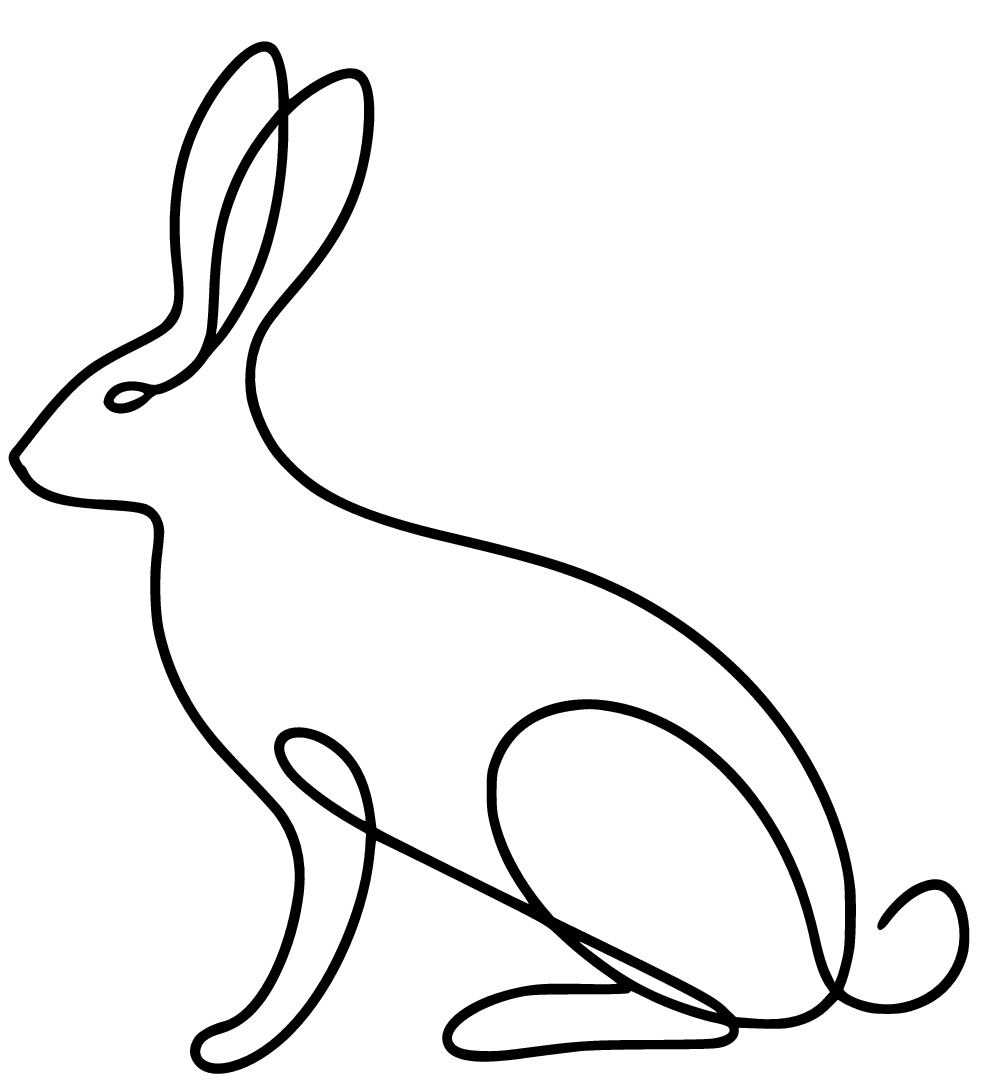
\includegraphics[width=0.15\textwidth]{images/fig_hare_.png}
    %\caption{The hare}
    \label{fig:hare}
\end{figure}

Below the signature, in the space left at the bottom of the page, something moved.

Celine leaned closer, holding the lamp low over the paper. A hare --- small, perfectly observed, rendered in a handful of sure lines --- was making its way across the lower margin of the letter. It moved with the particular lightness of a hare at speed, ears flat, hindquarters driving, each hop covering the distance with an ease that made the small space of the page seem briefly larger than it was. It reached the edge, paused for a fraction of a second as though considering, and then turned and came back the other way, unhurried now, stopping once to sit up and look at nothing before continuing its circuit.

Celine watched it for a long moment without speaking.

\enquote{I like her already,} she said.

Cecile looked at the letter, then at the sleeping figure in the upper berth, then back at the hare still making its quiet rounds at the bottom of the page.

\enquote{Yes,} she said. \enquote{So do I.}

\section*{The Changed Motion}

Thomas was not sure what woke him. Not a sound exactly --- more the absence of the rhythm he had fallen asleep to. The Siren had found a steady motion somewhere in the Irish Sea, a long, rolling movement that had lulled him under almost immediately after his head touched the pillow. Now that motion was gone, replaced by a shorter, more erratic rhythm, the ship climbing and dropping in a way that suggested the sea had changed its mind about the whole arrangement.

He lay still for a moment, listening. Rain, heavy and insistent, against the deck above. The groan of timber under stress. Pippin shifting on his hook, feathers rustling in the dark.

He climbed down from his berth.

Baldwin was already awake, sitting on the edge of his lower berth with his spectacles on, which meant he had been awake for some time. He looked up when Thomas's feet hit the floor.

\enquote{Rough,} Baldwin said.

\enquote{Yes,} Thomas agreed.

They dressed without much discussion and made their way up to the common room.

It was empty of students. The enchanted ceiling was doing its best with difficult material --- a dark, turbulent sky, the stars entirely gone behind cloud, the golden constellations absent for the first time since they had boarded. The lamps swung on their brackets with every roll of the ship. At the far end of the room, near the door that led to the sterncastle, Headmaster Hepburn was standing with the captain, both men leaning over the navigation table, speaking in low voices.

Thomas and Baldwin took the nearest bench and sat down quietly. Neither man had noticed them.

\enquote{--- can't hold this heading much longer,} the captain was saying. His voice was the voice of someone delivering an assessment rather than a complaint, precise and without drama. \enquote{Visibility is gone. I can't see the coastal lights and I won't risk moving in closer to find them. Not in this.}

\enquote{How far are we from the passage?} Hepburn asked.

\enquote{Far enough that it matters.} The captain straightened. \enquote{We need guidance, Headmaster. The stars are covered and the lights are useless to us. If we sit here we lose time we don't have, and if we move blind we risk the rocks.}

Hepburn was quiet for a moment. Thomas watched him think --- the headmaster's broad face still, his eyes on the navigation table without really looking at it.

\enquote{The selkies,} Hepburn said.

The captain nodded once, as though this was the answer he had been waiting for someone else to say first. \enquote{It's that or we anchor and wait out the storm. Which could be two days.}

\enquote{We can't wait two days.} Hepburn straightened and reached for his wand. \enquote{Wake the staff. I want every first and second year student in this room. As quickly as you can manage it.}

Thomas and Baldwin looked at each other.

\enquote{Selkies,} Baldwin said, quietly enough that it didn't carry.

\enquote{You know what they are?} Thomas asked.

\enquote{I've read about them.} Baldwin pushed his spectacles up. \enquote{Not much. The sources I found weren't particularly ---} he paused, searching for the right word, \enquote{--- convinced they were real.}

\enquote{They apparently are,} Thomas said.

They didn't have to wait long. Philippa arrived first, which surprised no one who had spent any time around Philippa --- she appeared to have been fully dressed already, her blue eyes alert, taking in the navigation table and the two men and the general atmosphere of controlled urgency with the rapid assessment of someone who had grown up around merchant emergencies.

\enquote{What's happened?} she asked, sitting down across from them.

Thomas opened his mouth. Baldwin got there first, turning on the bench to face her and launching into a precise, slightly breathless account of everything they had overheard, in sequence, with very little editorialising. He had the manner of someone who had spent years in a bookshop absorbing information and had been waiting for a situation that required it.

He was halfway through when Celine appeared in the doorway, her sister a step behind her. Celine was still in her nightclothes, a heavy wool blanket pulled around her shoulders, her hair loose and her expression suggesting she had been woken from deep sleep and had come anyway without stopping to argue about it. Cecile was dressed, but only just, and was looking around the room with the careful attention she brought to everything.

They sat down. Baldwin, with minimal prompting, repeated himself from the beginning.

Philippa and Celine both looked at Cecile when he reached the part about the selkies.

Cecile shook her head slightly. \enquote{Don't look at me. Both my previous journeys were entirely uneventful. I've never heard of this being done.} She considered for a moment. \enquote{Which I suppose means it doesn't happen often.}

\section*{All First and Second Years}

The room filled gradually after that. Students arrived in ones and twos, some dressed and some not, all carrying the slightly dazed quality of people assembled by authority in the middle of the night. Thomas watched them come in, putting names to faces where he could --- Mæve Medici arrived with her herb pouch already in her hand, which suggested that whatever she had been doing before the summons, sleeping had not been part of it. Cassian Sterling came in looking not at the people around him but upward, at the empty ceiling where the constellations should have been, with the expression of someone personally affronted by the cloud cover.

And then a boy Thomas hadn't yet met came through the door, and the room was slightly different for it.

He was flamboyant --- there was no other word that fit as precisely --- not in the manner of someone demanding attention but in the manner of someone so entirely himself that attention followed as a natural consequence. He wore his robes with a deep green scarf wound at his neck, and he moved through the filling room with an unhurried ease, finding a place to stand near the port windows and looking out at the darkness beyond the glass with the focused interest of someone who intended to understand what he was looking at. Beside him, a girl with dark hair and a smudge of charcoal on her cheekbone was already doing the same --- not looking at the people arriving around her but at the swinging lamps, the shifting ceiling, the room itself. She had a sketchbook under her arm.

Hepburn waited until the movement settled, then raised his voice.

\enquote{Thank you for coming. I'll be brief.} He explained the situation in the same direct terms he had used with the captain --- the weather, the visibility, the risk of the rocks, the need for guidance that the ship's instruments couldn't provide in these conditions. \enquote{Selkies know these waters,} he said. \enquote{They can guide us through safely. But calling them requires a chant, and selkies are more responsive to younger voices --- they find them closer to their own nature. That's why you're here.}

He moved through the room distributing strips of parchment. \enquote{The Latin portion, all of you should manage. The Gaelic ---} he paused, scanning the room, \enquote{--- who among you knows it?}

Elara O'Connell raised her hand without hesitation. Two second-years followed --- a boy and a girl, Scottish by the look of them.

\enquote{Good.} Hepburn gave them a separate parchment. \enquote{You'll carry the second portion. Everyone else follows my lead on the Latin. We'll perform the chant in the lower hull, close to the water. Follow me.}

\section*{The Third Voice}

The lower hull was cold and close and smelled of tar and bilgewater and the sea pressing against the other side of the timber. The lamps down here were fewer, and the ones that were lit swung more dramatically than those above, throwing the curved walls into alternating light and shadow. The students pressed together in the available space, shoulders touching, the ship's movement more pronounced down here, more immediate.

Thomas kept one hand on a support beam. Beside him, Baldwin had his parchment raised to catch the lamp light.

Hepburn raised his hand. The room stilled.

They began.

The Latin came up first and it came up well --- twenty voices finding the rhythm together, filling the low space with something that felt purposeful and deliberate. Then the Gaelic rose beneath it, Elara's voice leading, the two second-years following, and for a moment the two portions found each other and became a single thing.

They finished. Hepburn raised his hand for silence.

They waited.

The hull spoke in its own language --- the long groan of stressed timber, the irregular knock of waves, the high thin whistle of wind through a gap somewhere above. Nothing else. No answer.

The captain, standing near the forward bulkhead, did not move. Hepburn's expression remained composed, but Thomas saw his eyes move sideways toward the captain and then back.

\enquote{Again,} Hepburn said.

The second attempt was bigger. Some of the students who had listened carefully the first time began to approximate the Gaelic phonetically, following Elara and the second-years by ear, shaping the sounds without understanding them, giving the chant more body. Thomas tried it himself, watching Elara's mouth and doing his best to follow. It felt clumsy and probably sounded worse, but the collective effort was real.

They finished. Hepburn held the silence again.

Nothing came back. The hull gave them only the storm.

The captain turned partially away and spoke in a low, rapid voice to his first mate. Hepburn was very still. The apprehension in the room no longer had to be looked for — it had weight and temperature, pressing in alongside the cold.

Thomas looked at his parchment. The Latin was correct. He had pronounced it correctly. It hadn't been enough the first time and it hadn't been enough the second time, and he didn't know what the third time would do differently.

Then Reza Pahrs began to sing.

He wasn't singing the words. He had no Gaelic, clearly, and he wasn't attempting to pronounce it either. He was singing the notes of the Gaelic portion --- the melodic line that ran underneath the words, separated from its text entirely, as though he had listened twice and quietly removed the music from its container. He started low, in a register that was velvet smooth, each note placed with an unhurried certainty. Then the line rose, and somewhere in the upper register there was a quality that was not quite roughness but not smoothness either --- a texture, like the grain in worked wood. Both qualities present, neither cancelling the other.

Elara turned toward him slowly, her expression unguarded, entirely caught off balance. She studied him the way she studied an exquisite work of art — not as a mystery to be solved, but as a thing worth simply appreciating.

One by one the other voices fell into place, not from confusion but because something had changed in the room and everyone felt it, the way you feel a shift in pressure before weather arrives.

Reza sang on. He found something beneath the melodic line --- a second thread, lower, offered rather than stated, patient --- and the two lines moved together in the close, lamp-lit space of the hull.

The answer came almost immediately.

Three sharp knocks, low and resonant and entirely deliberate, from the port side of the hull. A pause. Then two more, further forward. Then a long, slow sequence running from the bow toward midship, measured and clear, like a hand moving purposefully along the outside of the timber.

Hepburn's face changed. The relief on it was complete and immediate, a man setting down a heavy apprehension he had been carrying without showing it. Around him, the crew straightened collectively, the tension leaving their shoulders all at once.

\enquote{Starboard,} Hepburn said, already moving toward the captain. \enquote{Two knocks, turn to starboard. Take her around.}

The captain was already calling upward through the hatch, his voice carrying the same precision it had in the common room, unhurried and exact. Above them, the ship began to move differently.

Reza had stopped singing. He was listening to the last of the knocking with his head tilted slightly, a look of quiet attention on his face.

Elara was still watching him. \enquote{How did you know to do that?}

He turned to her. \enquote{They just like good music, darling.}

\section*{The Stone Coin}

Hepburn sent them upstairs while the crew worked. The common room was warmer than the hull and the ceiling had shifted during their absence --- the storm sky still dark and roiling, but the enchanted light of the lamps seemed to have registered the change in the room's mood, burning a fraction steadier than before.

They gathered at the familiar table by the window. Bread had been laid out, and butter, and a basket of apples from Dublin, and the pot of hot water with herbs beside it. Outside the glass, the sea remained invisible, the rain moving in long sheets across the darkness.

Thomas poured himself a cup of barley water and sat down. From below, muffled through two decks of timber, came two measured knocks --- a correction to the heading, perhaps, or a warning passed and heeded. The sound was distant but clear, and reassuring in a way he hadn't expected.

Baldwin had been quiet since they came up the stairs. He was doing his thinking face --- spectacles pushed up, hands around his cup, eyes focused on something slightly in front of him rather than the room.

Reza sat down across from Elara without particular ceremony, unwinding his scarf slightly in the warmth. Elara had opened her sketchbook on the table beside her bread and was looking at a page she had apparently filled during the night --- the hull's curved timbers, the swinging lamps, a few quick lines that suggested the shape of the storm outside without depicting it directly.

\enquote{I'm Reza,} he said, to her and to the table generally.

Elara looked up. She introduced herself, then worked around the table --- Thomas, Baldwin, Philippa, Celine, Cecile --- and Reza acknowledged each name with a nod that was brief and attentive, filing them away properly.

\enquote{I knew selkies existed,} Baldwin said suddenly, not quite to anyone. \enquote{I'd read about them. The sources I found called it folklore.} He paused. \enquote{The sources were wrong.}

\enquote{The sources always call it folklore,} Elara said, tearing a piece of bread. \enquote{In Ireland we don't need to write it down to know it's true.}

\enquote{What do you know about them?} Thomas asked her.

She considered, the bread held loosely in her fingers. \enquote{They live in the sea. They can shed the seal skin and take human form on land. They're not dangerous unless they've been wronged. They don't particularly seek out wizards --- they have their own concerns, which are older than ours.} She glanced at Baldwin. \enquote{They can be called in the old way, when the need is genuine and the call is made properly. They come because they choose to. Not because they're obliged to.}

\enquote{But they came,} Celine said.

\enquote{The call was right, eventually.} Elara looked at Reza briefly, then back at her bread.

\enquote{I've read that there are formal arrangements,} Baldwin said, thinking aloud. \enquote{Between the wizarding world and ---} He stopped. The door from the corridor had opened.

The selkie came in without announcement, and the room rearranged itself around him the way a room does when something enters that belongs to a different set of rules. He was lean, with black hair and pale skin and bare feet that left faint damp prints on the wooden floor. He wore a simple linen tunic under a seal skin draped across one shoulder. He was slightly wet and entirely unbothered by it. His eyes moved across the room once, taking everything in, and then settled on Hepburn.

Hepburn rose. He crossed the room with a respect that was not the formal courtesy he might extend to a visiting dignitary but quieter and more considered. He drew his wand.

\enquote{What is he doing?} Philippa asked under her breath.

\enquote{Watch,} Elara said.

Hepburn produced a Galleon from his coat, held it up briefly, and set it on the table between them. He touched it once with his wand. The gold shifted, dulled, lost its warmth, and became stone --- the same shape and markings as before, but grey and cold and heavy-looking where it had been bright a moment ago.

The selkie looked at it. He picked it up.

\enquote{That stone,} Baldwin said slowly, working it through as he spoke, \enquote{is ---}

\enquote{An obligation,} Elara said. \enquote{The wizarding council made it mandatory. If a selkie presents that stone to a wizard, that wizard is required to provide assistance. Not asked. Required. The closest wizard to them when they show it is bound to help --- there's no refusal. No choice.} She paused. \enquote{After the help is given, the stone turns back to gold. That's the payment.}

\enquote{So the gold is the end of the debt,} Philippa said, watching Hepburn.

\enquote{The stone is the debt,} Elara said. \enquote{The gold closes it.}

The selkie held the stone coin in his closed hand for a moment. Then he inclined his head toward Hepburn --- not quite a bow, but carrying the same weight as one, an acknowledgment between parties who regarded each other as worth the formality. Hepburn returned it.

The selkie turned toward the door.

At the threshold he paused --- not long, barely a full second --- and his gaze moved back across the room. It found Reza, who was sitting with his cup and his green scarf, watching the whole thing with calm, interest and intent to remember it. The selkie looked at him. Just looked, for that fraction of a second --- the particular recognition of one creature for another who has done something worth acknowledging --- and then he was gone.

The door settled shut behind him.

From below, distant and clear, a single long knock sounded against the hull. Then silence. The ship moved steadily beneath them, and outside the rain continued, but the quality of the movement had changed --- purposeful now, guided, finding its way through the dark with something alongside it that knew the water and the rocks and the shape of the passage ahead.

Celine let out a slow breath.

\enquote{Well,} said Reza, picking up his cup at last. \enquote{That was a very good morning.}
